\documentclass{article}
\usepackage[utf8]{inputenc}
\usepackage[english]{babel}
\usepackage[utf8]{inputenc}
\usepackage{fancyhdr}
\usepackage{graphicx}
\usepackage[toc,page]{appendix}
\usepackage{multicol}


\title{SLM Circuit Simulator Log}
\author{Sam Taylor, Maximus Wickham , Leonardo Garofalo}
\date{June 2020}

\pagestyle{fancy}
\fancyhf{}
\rhead{SLM Soloutions}
\lhead{SLM Circuit Sim}
\rfoot{Page \thepage}

\graphicspath{ {./images/} }
\begin{document}

\maketitle
\newpage
\tableofcontents
\newpage

\section{Engineering Design Process}
\flushleft

\subsection{Outline of technical problem to be solved:}
\flushleft

\smallbreak
Write a software package that performs a transient simulation of a circuit, like LTspice. The main elements of such a system are described below:
\newline
\smallbreak
1. Parse the netlist file using reduced SPICE format.
\newline
2. Set up the simulation (Transient Analysis , DC Bias Point Analysis)
\newline
3. Construct and solve the conductance matrix
\newline
4. Process voltage sources
\newline
5. Write the output
\newline
6. Add support for non-linear components (advanced)
\newline
\mediumbreak 

Key Evaluation points:
\newline
1. Accuracy: compare the outputs to pen and paper solutions. 
\newline
2. Efficiency: find how long the simulation takes and, by estimating the power consumption of your computer.

\subsection{Software Requirements Specification:}
\flushleft
\textbf{Outline:} A circuit Simulation that produces transient analysis for circuits containing energy storage devices , diodes and transistors . With reasonable accuracy and speed.

\bigbreak

\textbf{Functional Requirements}

\newline

1. Give Node Voltages of a complete circuit within 1 percent of Spice
\newline
2. Evaluate Current flowing through each component within 1 percent of Spice
\newline
3. Perform analysis for passive, energy storage devices , diodes and transistors.
\newline
4. Take input from a reduced spice netlist file.
\newline
5. Output analysis to an output file.
\newline
6. The software must be capable of dealing with both linear and non-linear devices

\bigbreak

\textbf{Non-Functional Requirements}
\newline
1.The software must be capable of analyse different kinds of circuits
\newline
2. The software must be able to perform the analysis in a fast and efficient way
\newline
3. The software must be capable of performing the analysis consuming the least amount of power possible

\newpage

\subsection{Overview of Design}
\textbf{Data Flow / Structure}
\newline
The input net list is in the form of a txt file with two output files: output\verb|_|current and output\verb|_|voltage . The output files are in a CSV format with each line denoting a time instance. The parser creates a circuit object passes that as well as the transient time step and time period. Transient analysis then loops through the Transient solver recursively performing KCL solver. From this we agreed upon data inputs and outputs to each function.

\begin{figure}[h]
    \caption{Overview of data flow}
    \centering
    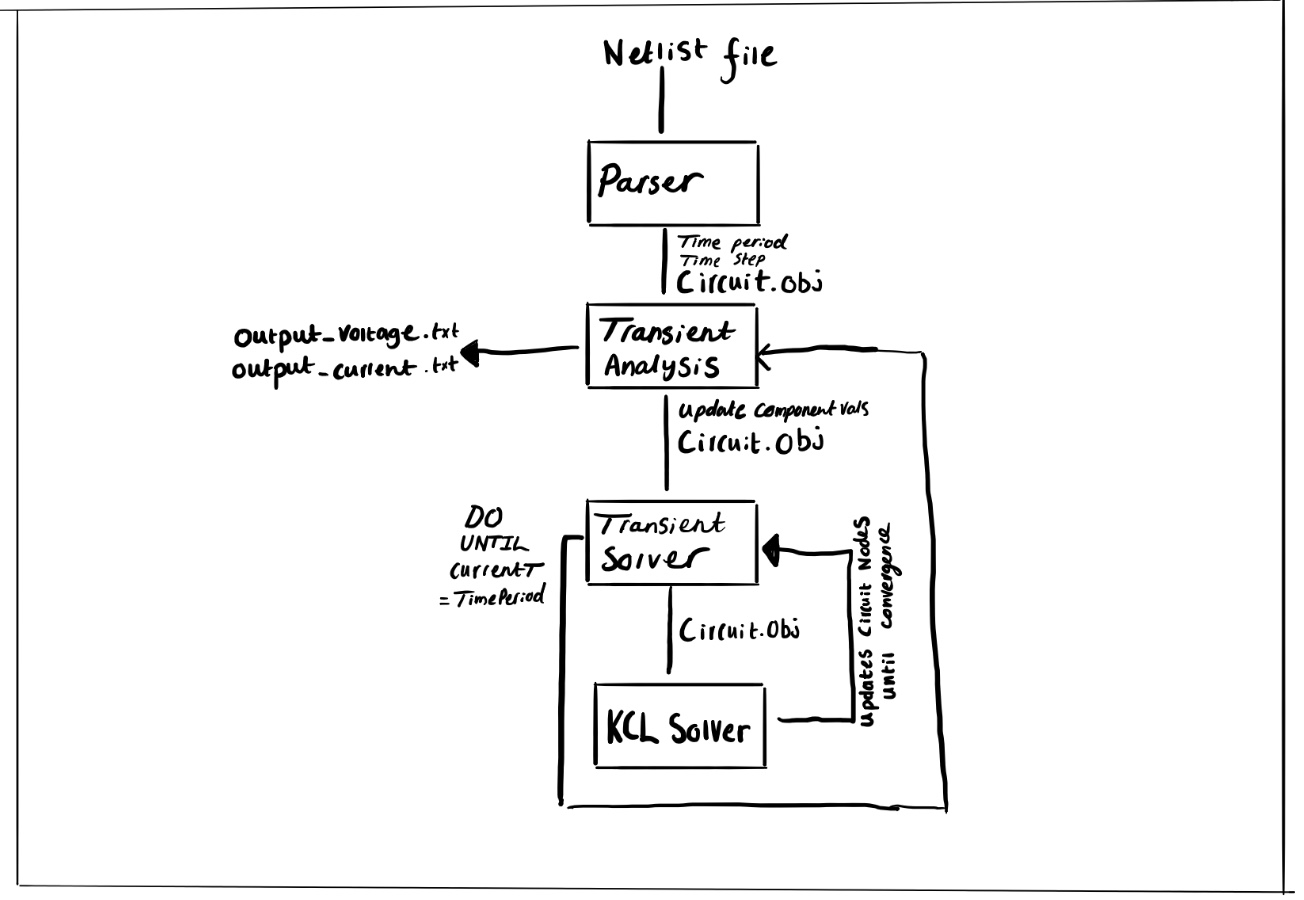
\includegraphics[width=\textwidth]{images/Comphpp.jpg}
    \label{fig:AlgoOverview}
\end{figure}

FILL ME IN WITH MORE DESIGN

\newpage

\subsection{Design Process and Project management}

We chose to use the Scrum framework to manage our collaboration during the project. We initially populated the project backlog with details from the specification and our design overview. Each morning (at varying times) we held a thirty minute scrum to inform each other what we work we would be doing that day. At the end of each day we held a second meeting to discuss what was achieved and what problems we encountered updating the backlog with completed and new tasks.
We also held a bi-weekly sprint meeting where we determined the milestone and objectives of that sprint. We did not use a sprint backlog just kept a single updated backlog. 

\begin{figure}[h]
    \caption{Scrum Framework work pattern}
    \centering
    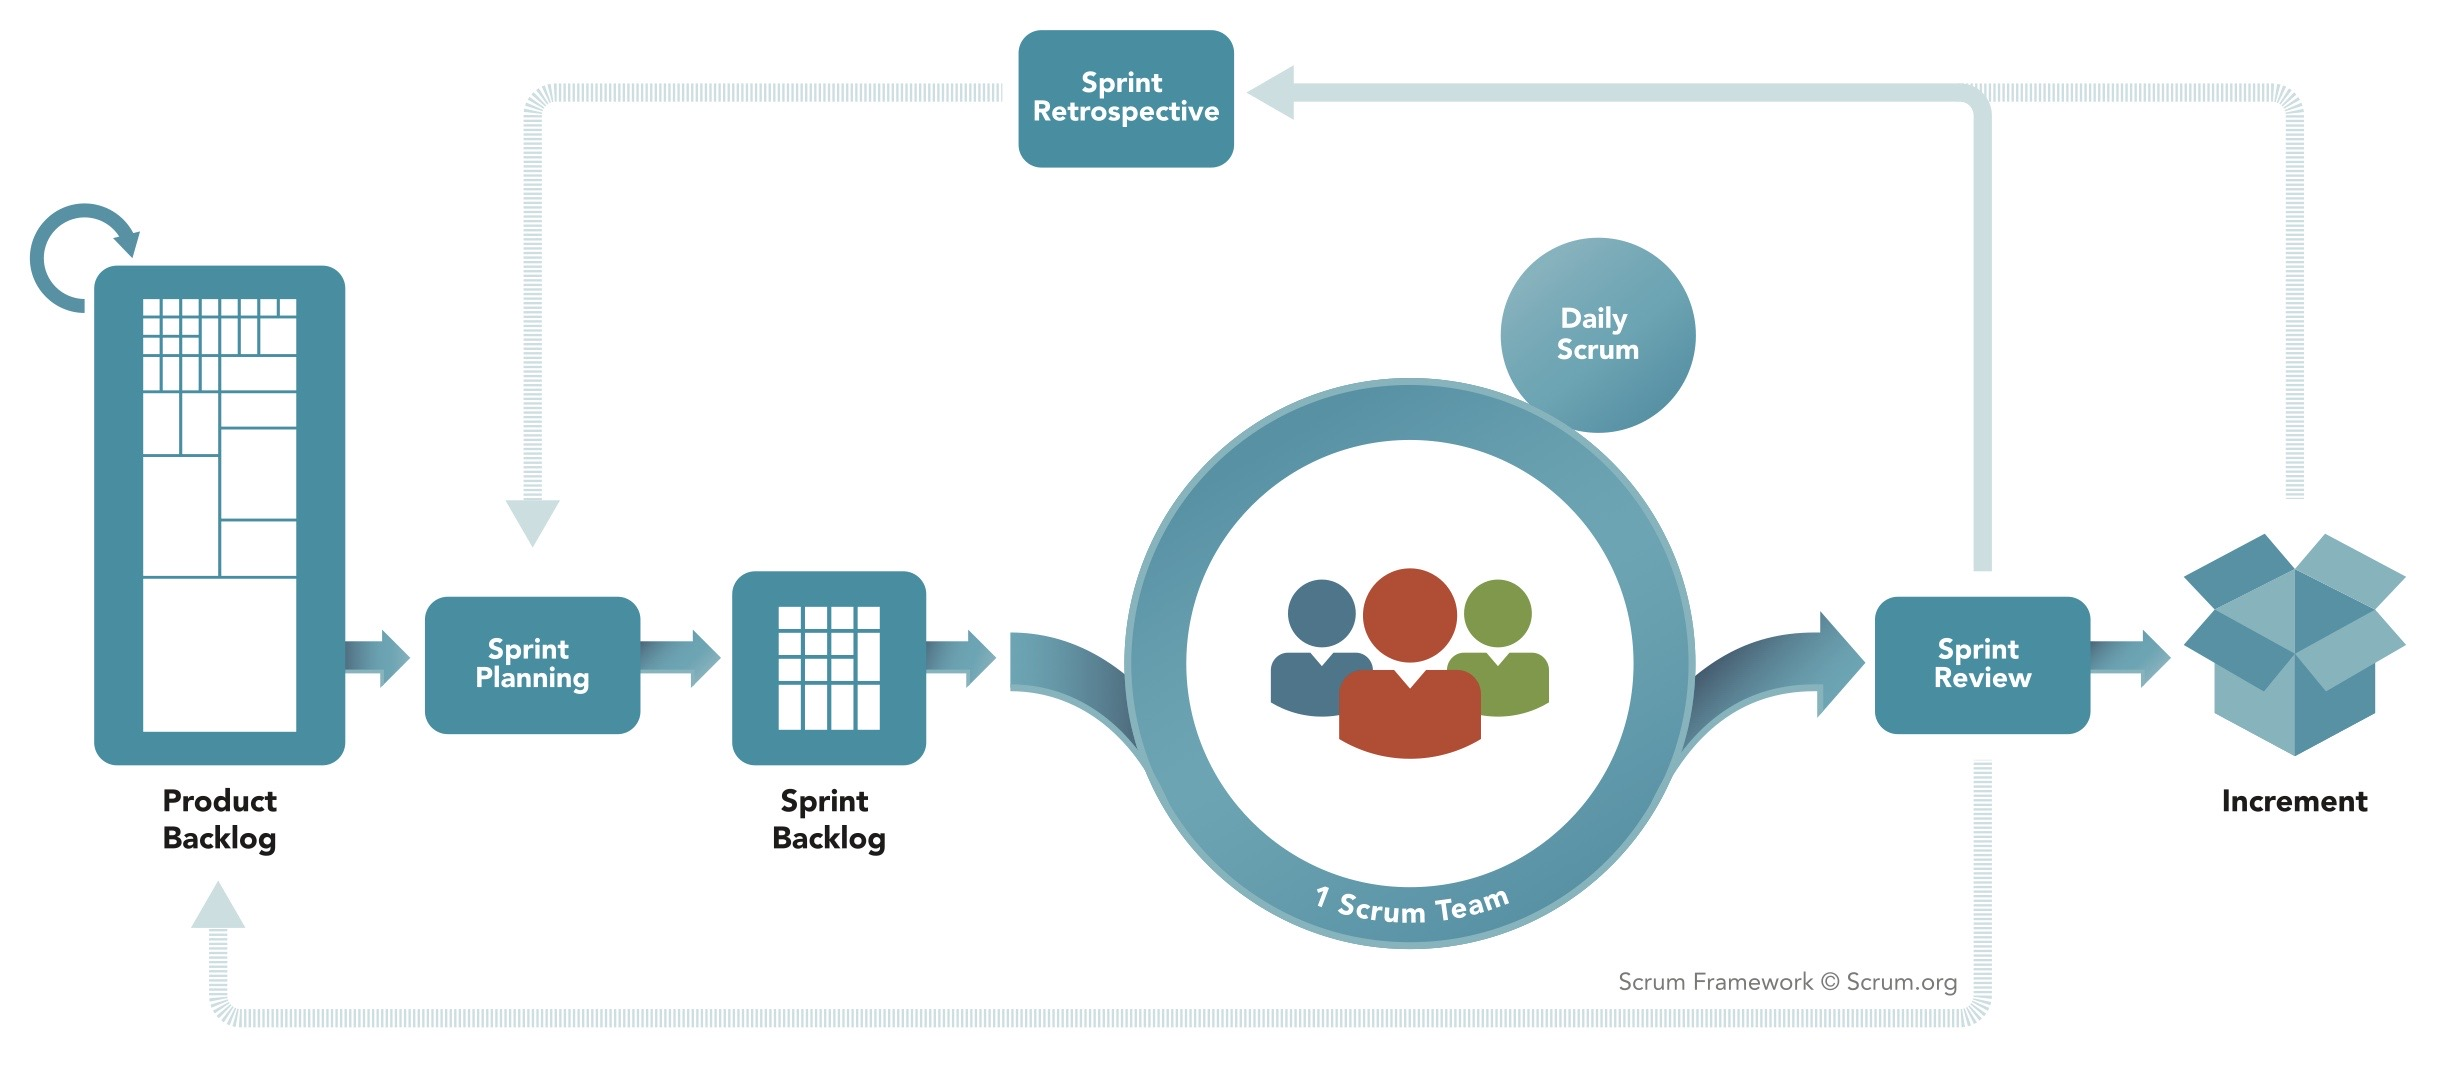
\includegraphics[width=\textwidth]{images/ScrumFramework.jpg}
    \label{fig:Scrum}
\end{figure}
We also used a timeline to keep general project discipline and keep goals realistic to the final deadline. This was used to ensure we were not implementing more functionality beyond our ability to produce a write up.
\begin{figure}[h]
    \caption{Snapshot of Onenote backlog}
    \centering
    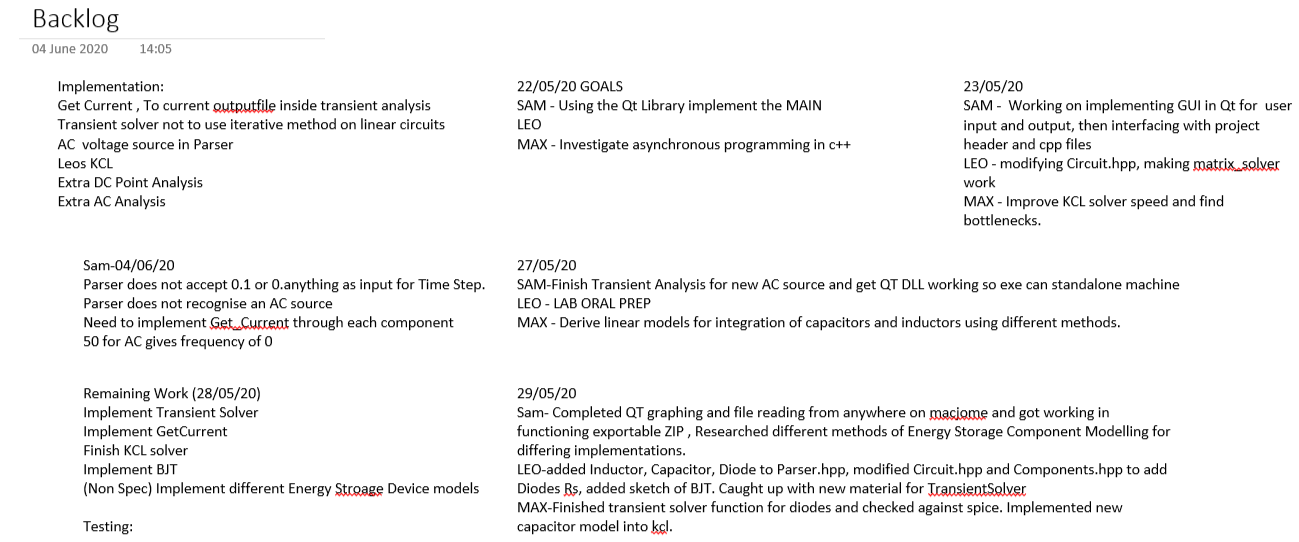
\includegraphics[width=12cm]{images/Backlog.PNG}
    \label{fig:BackLog}
\end{figure}

\newpage

\subsection{Design Process Review}



\newpage



\section{Component Models}
The following section will go through the models and implementations for each Electrical component in our simulation.
\begin{figure}[h]
    \caption{Component Inheritance tree}
    \centering
    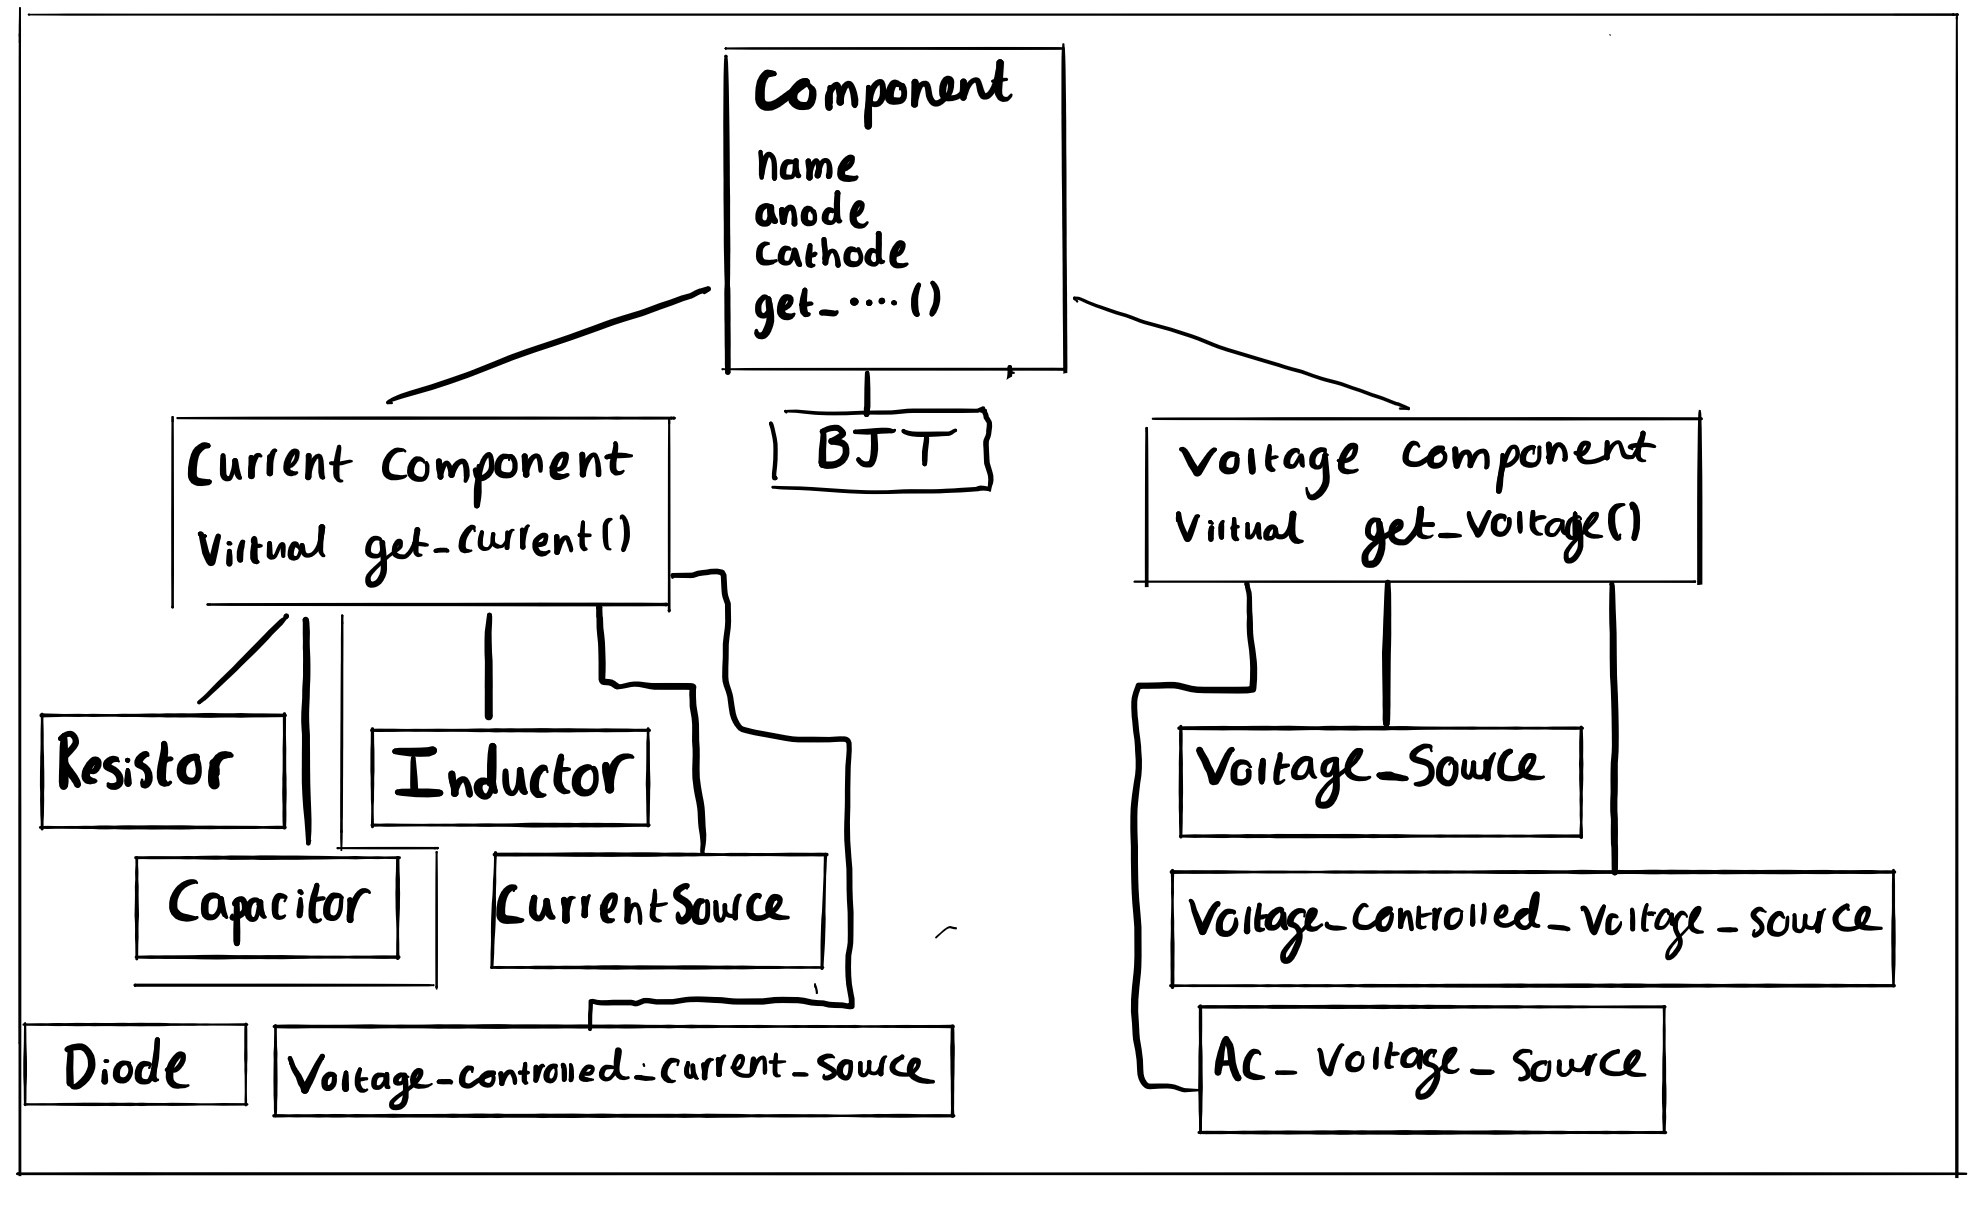
\includegraphics[width=12cm]{images/Comphpp1.jpg}
    \label{fig:Comp}
\end{figure}

\subsection{Current Components}
Current components , have virtual function called get\verb|_|current() that allows the any component that is a current component to be cast into a current component and have its get\verb|_|current function called , conveniently allowing differentiation between components of different properties in KCL solver and avoiding needless selection.
\bigbreak
See Appendix A (Current Components) for implementation
\medbreak


\subsubsection{Resistor}
The resistor is a simple component to implement with respect to our design hence a simple self produced model was used. The class contained a resistance and conductance variables and a get\verb|_|current method which took the node voltages and resistance of the component. \bigbreak\\$Current = \frac{VAnode - VCathode}{R}$
\bigbreak
See Appendix A (Resistor) for implementation
\newpage
\subsubsection{Capacitor}
The capacitor is an energy storage component , hence the transient analysis of such a component requires the use of a companion model to be formed. Multiple were researched that can represent both the capacitor: Backward Euler , Forward Euler and Trapezoidal Rule. It is possible to derive the next voltage of a capacitor from its differential equation:
\bigbreak\\$I= C\frac{dv}{dt}$
\bigbreak
$ v(t + \Delta t)= v(t) +  $\frac{1}{C}$ $$\int_{t}^{t+\Delta t} i(u) du$$ $

\bigbreak

Thus we can interpet this simplified equation into a (Norton????OR THEVENIN) form companion model, that gives us: 

\bigbreak

\begin{multicols}{2}
\noindent
  \begin{equation}
    Conductance = \frac{C}{\Delta t}
  \end{equation}
  \begin{equation}\break
    LinearCurrent = \frac{Conductance}{V_n}
  \end{equation}
\end{multicols}


\newpage

\subsubsection{Inductor}
\newpage

\subsubsection{Current Source}
\subsubsection{Voltage Controlled Current Source}

\subsection{Voltage Components}
Voltage components , have virtual function called get\verb|_|Voltage() that allows the any component that is a voltage component to be cast into a voltage component and have its get\verb|_|Voltage() function called , conveniently allowing differentiation between components of different properties in KCL solver and avoiding needless selection.
\medbreak



\subsubsection{Voltage Source}
\subsubsection{Voltage Controlled Voltage Source}
\subsubsection{AC Voltage Source}
\newpage

\subsection{Semiconductor Components}
\subsubsection{Diode}
Unlike the other components discussed so far, diodes do not have a linear relationship between voltage and current. This means that using a linear matrix method to solve the circuit would not be possible when non-linear components such as diodes are present. However, due to the exponential formula for the current through a diode an analytical solution is often far too complex and even impossible. Therefore, the iterative Newton-Raphson technique for solving equations had to be used. This algorithm is discussed in detail in the Transient Solver section, with it resulting in a linear implementation of the diode component.
\\
Inside SPICE the current equation of a diode is dependent on several parameters. 
\begin{itemize}
    \item Is
    \item N
    \item BV
    \item Rs
    \item GMIN (universal constant)
\end{itemize}
Using these parameters the current through the diode is broken down into three sections. When the voltage across the diode is greater than $-5NVt$ (where $Vt = kT/q$ and is taken universally within the simulator to be 0.0258641) the equation is the standard Shockley equation.\bigbreak \\ $I = Is*(e^{\frac{Vd}{N*Vt}}-1) + Vd*GMIN$. \\\bigbreak GMIN is simply the min conductance of the diode and represents a resistor in parallel to it aiding in convergence. When Vd is less than $-5NVt$ but greater than BV the exponential is not worked out as it is insignificant next to the effect of GMIN. BV represents the breakdown voltage of the diode and when VD is less than it the equation is modified.\bigbreak
\\$I = -Is*(e^{-\frac{BV+Vd}{N*Vt}}-1+\frac{BV}{Vt})$\\\bigbreak
The value Rs represents the connection resistances of the diode and is equivalent to a resistor in series with the diode described by these equations. The diode that is implemented in our simulator is the 1N194 and has values taken from LTspice of $Is=2.5n$, $Rs=0.568$, $N=1.752$ and $BV = -70$.  
\\
In order for the iterative technique to be implemented an ideal diode has to be implemented as a current source in parallel with a resistor, as any linear voltage current relationship can be simplified to this. It would be possible to represent the diode as a voltage source and resistor in parallel but this would make generating matrix coefficient harder due to the presence of an extra node. It would also be slower due to voltage sources being more complex to compute in our matrix solver algorithm. Three functions had to be implemented to set the values of the current source and resister which were as follows.
\begin{itemize}
    \item Set Vd (double \_vd)
    \item Set id0 (double (\_ido)
    \item Set Conductance
\end{itemize}

Set Vd and Set ido are simply needed to set the current through the diode and voltage across it at the last iteration. Set Conductance is needed to set the conductance of the resistor in the linear model. This had to be equal to the partial derivative of the diode current equation with respect to voltage. This partial derivative is broken down into three sections to match the current equation described above with the section relating to the Shockley equation as follows.\bigbreak
\\$G = \frac{Is}{N*Vt}*e^{\frac{Vd}{N*Vt}}$\\\bigbreak
Unfortunately, the conductance and linear current of the diode could not be used immediately inside of the KCL solver algorithm. This is due to the presence of the a series resister in the diode model. One approach to this problem could have been to add a resistor in series with the diode in the circuit, but this would have added another node thus increasing the complexity of our matrix and slowing down the simulation. Instead the dependence of the current through the diode on the voltage at each node is calculated as well as the constant current emitted by it. Three functions were made to implement this. 
\begin{itemize}
    \item Get Anode Coefficient
    \item Get Cathode Coefficient
    \item Get Constant Coefficient
\end{itemize}
The outputs of these function can be read directly into the conductance matrix and current vector within the KCL algorithm. The derivation for these values is shown using the circuit in figure \ref{fig:diode}\bigbreak
\\$(V_0-V_1)*G_s = (V_1-V_2)*G_l - I_l$\bigbreak
\\$V_1 = \frac{V_0*G_s + V_2*G_l - I_l}{G_s+G_l}$\bigbreak
\\And so the current passing through $G_s$ is given by:\bigbreak
\\$V_0*Gs - \frac{V_0*G_s^2}{G_s+G_r} - \frac{V_2*G_r*G_s}{G_s+G_r} + \frac{I_l*G_s}{G_s+G_r}$\bigbreak
\\Thus the coefficients can be taken from this equation. \bigbreak
\\$V_0$ coefficient is given by $Gs - \frac{G_s^2}{G_s+G_r}$\bigbreak
\\$V_2$ coefficient is given by $- \frac{G_r*G_s}{G_s+G_r}$\bigbreak
\\The constant coefficient is given by $\frac{I_l*G_s}{G_s+G_r}$\bigbreak
These three terms completely describe the diode model with the KCL solver algorithm as the GMIN value is added to the value of $G_l$. The presence of this series diode presents another problem though. In order for the linear current and conductance to be set by the Transient Solver algorithm the voltage across the diode is needed. However, this is no-longer simply the voltage across the terminals due to the presence of Rs. In order to account for this when setting the voltage across the diode the voltage across Rs, calculated using the current through the diode is subtracted from the voltage between the nodes. 
\begin{figure}[h]
    \caption{Linear Model of Diode}
    \centering
    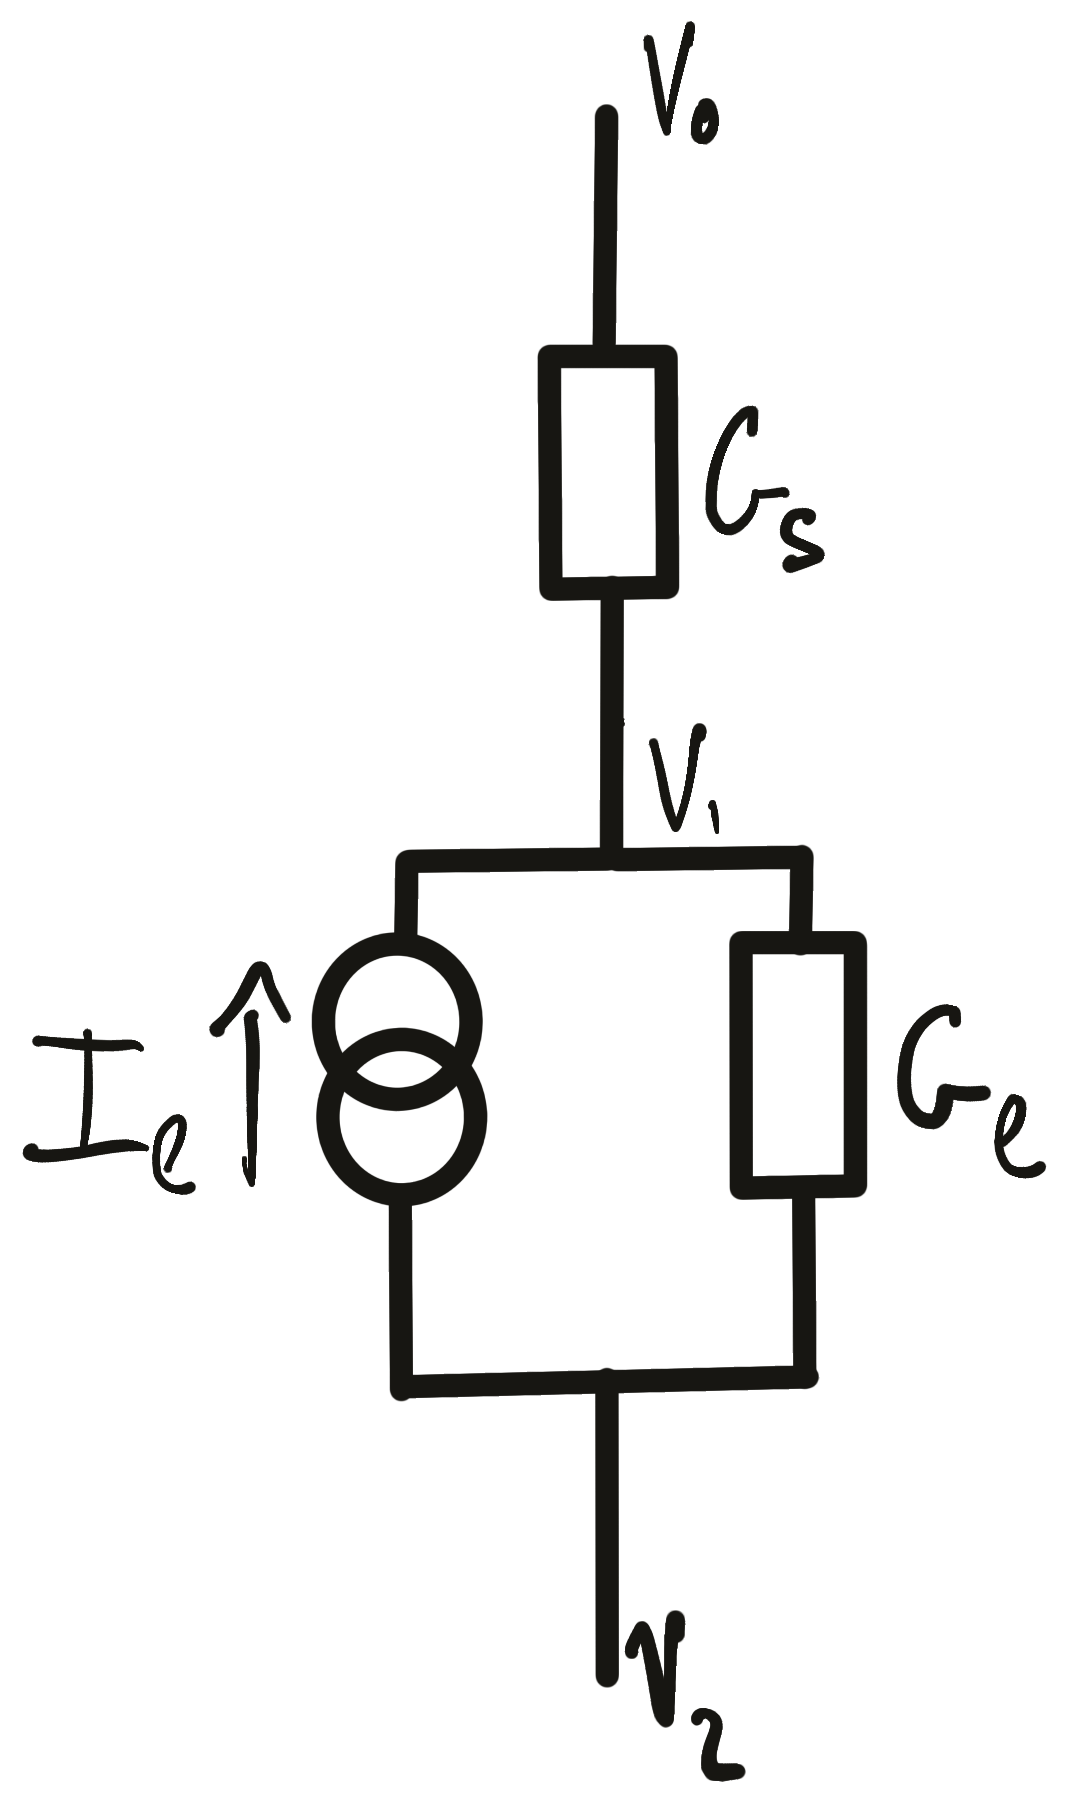
\includegraphics[width=0.25\textwidth]{images/DiodeCircuit.png}
    \label{fig:diode}
\end{figure}

\subsubsection{BJT}


\section{Analysis Algorithms}
\subsection{Parser}
\subsection{Transient Analysis}
\subsection{KCL Solver}
\newpage
\subsection{Transient Solver}
When non-linear components such as BJT's and diodes are present in a circuit solving the circuit using linear algebra is no-longer possible. Due to the complexity of diode and BJT equations the method used to solve these non-linear circuits is the iterative Newton-Raphson method. The equation that describes the iterative method is:
\bigbreak $x_{n+1} = x_n - \frac{f(x_n)}{f'(x_n)}$\bigbreak
By repeating this iteration $x_n$ may converge such that $f(x_n) = 0$
Originally we considered that due to the presence of many node voltages in a circuit and a diode current being dependent on two of those voltages a multi-variable method would have to be used. We researched how to modify the above equation for multi variable equations and found a lecture\cite{mulitvariableNR} describing the use of a Jacobian matrix. We tried implementing this method by giving each current component a function that returns a vector storing the partial derivatives of its current with respect to each current. However, we where never able to get this method to converge correctly with diodes, with the method also adding a lot of extra code and computation. Having tried this method we then found after more research that we could describe the current through the diode as a function of the voltage across it which is only one variable\cite{LinearCompanionModels}, so the use of multi-variable iteration was not needed. In order to solve the diode using Newton-Raphson we need to form an KCL equation that is equal to 0. Doing KCL at the diodes anode we have the equation:
\bigbreak $I_d - I_{in} = 0$\bigbreak
Where $I_in$ is the current entering the diode and $I_d$ is the current due to the diode current equation. Combining this with Newton-Raphson gives:
\bigbreak $x_{n+1} = x_n - \frac{I_d - I_{in}}{\frac{d I_d}{d V_d}}$\bigbreak
The Newton Raphson method the function each iteration as a linear function and so a diode is going to need to be modeled as a resistor and current source in parallel as any linear voltage current relationship can be modelled as this, (apart from those with an infinite gradient). I we consider a diode as a current source in parallel with a resistor we can again do KCL at its anode to form the equation. 
\bigbreak $V_d*G_l + I_l - I_{in} = 0$ Where $G_l$ and $I_l$ are the conductor and current source values.\bigbreak
We want to find a value of $G_l$ and $I_l$ such that if we solve the circuit using the KCL solver algorithm the voltage across the diode will be $V_{n+1}$
\bigbreak
Thus if we rearrange the Newton-Raphson equation we have:\bigbreak
$x_{n+1}*\frac{d I_d}{d V_d} = x_n*\frac{d I_d}{d V_d} - I_d + I_{in}$\bigbreak
From this we can see that if we make $G_l = \frac{d I_d}{d V_d}$ and $I_l = I_d - x_n*\frac{d I_d}{d V_d}$ when the equation is solved the voltage across the diode will be $V_{n+1}$\bigbreak
If we keep repeating this method of setting the value of G and I for each diode and then solving the circuit and then resetting the values the circuit should converge to the correct values. To complete the iterations though we need some way of telling when the circuit has converged to an acceptable accuracy. 
Within Spice two parameters are used to measure this convergence.
\begin{itemize}
    \item RELTOL
    \item ABSTOL
\end{itemize}
Spice combines these two parameters within the inequality $|v_{n+1}-x_n| < RELTOL*|x_n| + ABSTOL$.\\
RELTOL measures the relative change in the voltage and ABSTOL is present as near 0V $RELTOL*|x_n|$ may become too small. Each iteration of our algorithm each of the node voltages is compared using this inequality to the previous voltage and if all the inequalities return true the algorithm finishes. A maximum number of iterations is set so that the program can't get stuck in an infinite loop. Within our program the max iterations was set to 1000 as we found that a correct circuit usually has a max iterations of a few hundred on the first time step and so this provides room for that occur. We set RELTOL and ABSTOL to values of $10^{-3}$ and $10^{-12}$ respectively. This provided a trade off between accuracy and speed of our program. If higher accuracy is needed RELTOL should be decreased. 
\bigbreak
In order to implement this algorithm the flow diagram shown in figure \ref{fig:transient}. The entire algorithm is contained within one function called TransientSolver. This function takes a circuit object by reference and modifies its voltages to the correct voltages given components in the circuit or exits the program if the maximum iterations is reached. This means that the starting guess for the voltage is the voltages from the previous time instance meaning that they are very close to the new voltages. This results in very few iterations normally being needed. Only the first iteration with starting guesses of 0V takes many iterations under normal use. \\

The algorithm runs within a while loop, starting by looping through all the components and setting the linear current and conductance of all diodes and BJT's. As BJT's are simply modelled as containing two diodes they converge in the same manner as diodes do. The algorithm then saves the circuit voltages in a vector before running the KCL solver algorithm on the circuit. After this it compares the old voltages with new and breaks the while loop if complete.  

\begin{figure}[h]
    \caption{Transient Solver Algorithm}
    \centering
    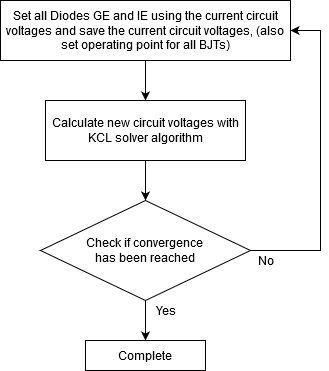
\includegraphics[width=0.5\textwidth]{images/TransientSolverAlgorithm.png}
    \label{fig:transient}
\end{figure}

\newpage

\section{Application Features and Innovation}
\subsection{QT Container and Application}
Biggest innovations: 
QT
Used derivations to eliminate mathematical complexity and faster implementation: In diode and BJT. 



\section{Testing and Evaluation}

\section{Final Evaluation}

\newpage



\bibliographystyle{plain}
\bibliography{bibliography.bib}

\appendix
\section{Appendix}
\textbf{Current Component}
\bigbreak
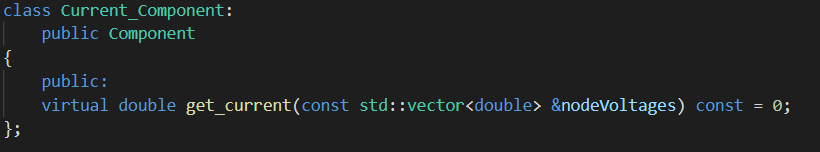
\includegraphics[width=12cm]{images/Current_Component.PNG}
\bigbreak
\textbf{Resistor}
\bigbreak
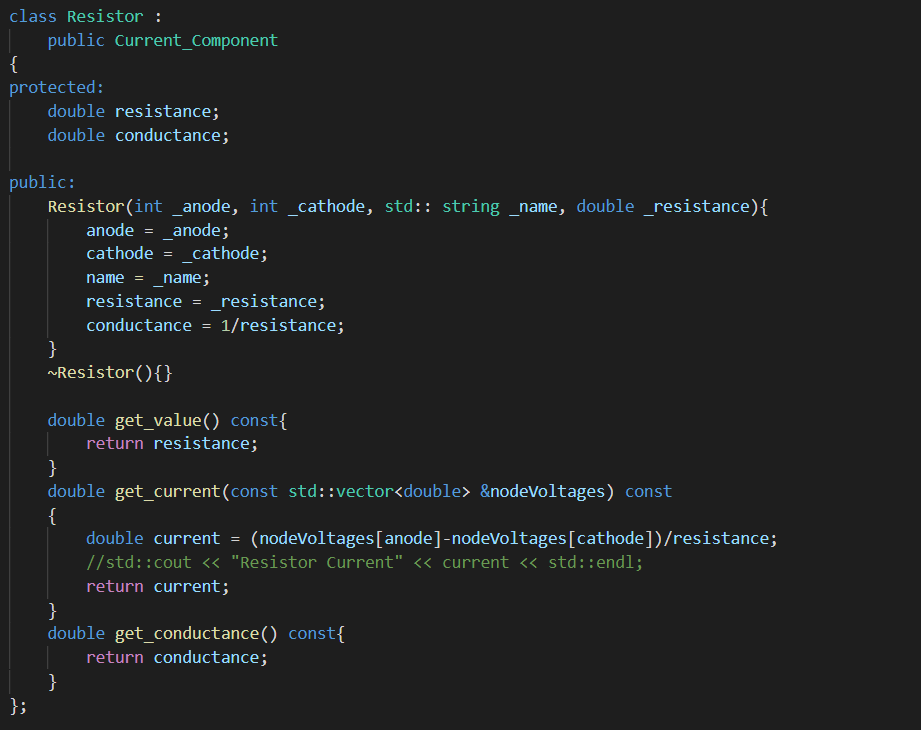
\includegraphics[width=12cm]{images/Resistor.PNG}
\bigbreak
\newpage
\textbf{Capacitor}
\bigbreak
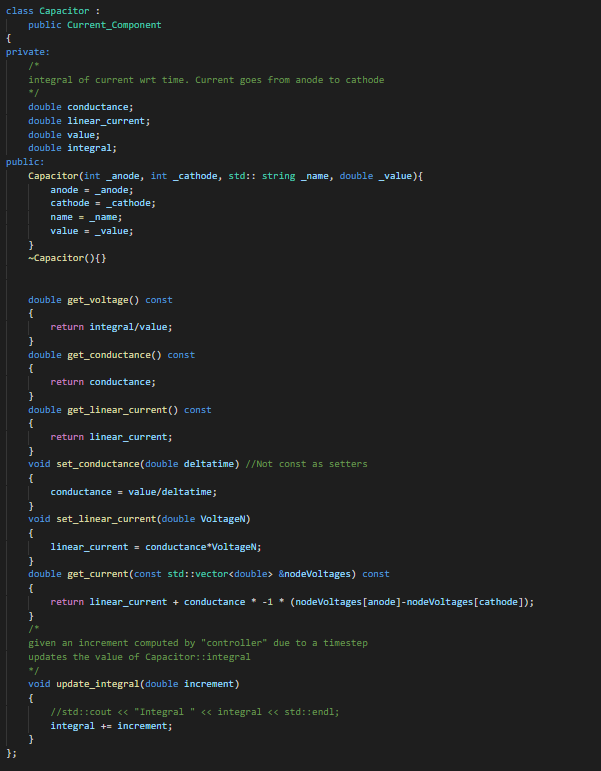
\includegraphics[width=12cm]{images/Capacitor.PNG}
\bigbreak
\newpage
\textbf{Inductor}
\bigbreak
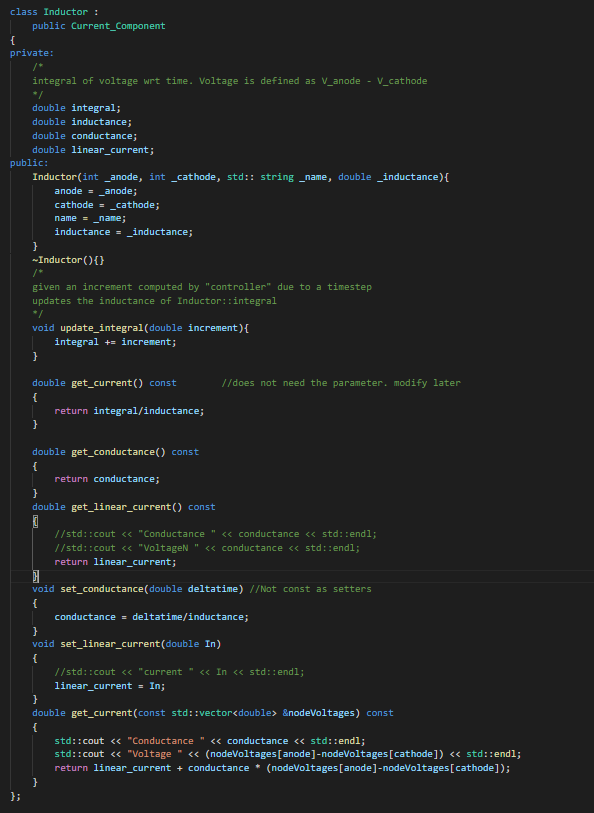
\includegraphics[width=12cm]{images/INDUCTOR.PNG}
\bigbreak

\end{document}
